\section{Integration}

\subsection{Parallelization}
The integration of the various components of our platform will be realized at the end of
the development process. This way we can parallelize the implementation, having different teams
independent from each other till the completion of their respective components.
All components will be unit tested to prevent common errors from being overlooked.
\newline
\newline
Whenever two components are integrated, specific integration tests will be written to
verify the end result.
\newline
\newline
Once the server and client application have been completed they will be integrated using REST APIs.
The process won't need any refactoring of the client application, as it will be developed using mock up classes and stubs for the server calls.
\newline
The client-server integration will need specific tests and human tests. We can take into consideration the
possibility of an early release of the application on the mobile application stores as a beta distribution
to collect a large number of feedbacks, regarding not only bugs and glitches of the client application but
also suggestions about possible improvements of the UX.

\subsection{External services}
Once our server application is completed and all its components have been successfully integrated,
we can start integrating external services to it.
\newline
\newline
We'll focus on the Cloud Storage solution first, because it's necessary to launch the client application.
The Cloud Storage solution will provide an HTTP API to access, modify and create multimedia content,
making our server a proxy to its data storage.
\newline
\newline
To integrate partners APIs we'll need to make specific agreements with each one of them. These
agreements will discuss the technicalities of their systems which may vary significantly from
one another.
\newline
\newline
Any possible municipality API for the retrieving of
statistical data about accidents will be integrated individually, due to the several differences
that can be found in each information system.
\newline
\newline
On the client-side a service that will be integrated in the first release is the map. Server-side we only need
to store the coordinates of the reports, latitude and longitude, while on the client-side these points will be presented
visually through a map service that accepts these parameters. 
This integration can be made independently of the server implementation process.

\newpage
\begin{figure}[H]
  \centering
  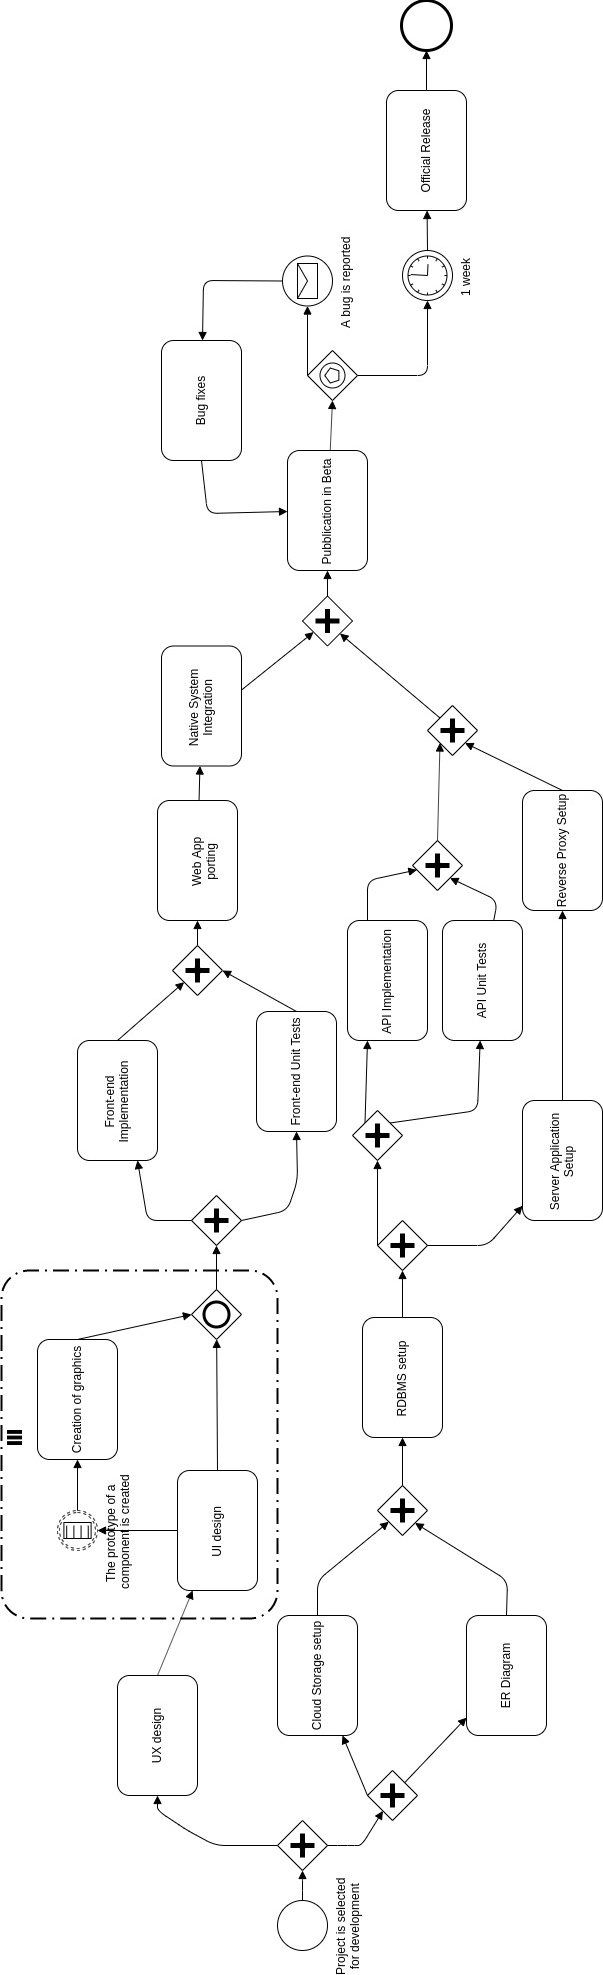
\includegraphics[origin=c,width=\textwidth,height=.95\textheight,keepaspectratio]{DD_Images/DevelopmentBPMN.jpg}
  \caption{\textit{Interface Diagram}}
\end{figure}